\Chapter{Pairings\label{hfdst-pairings}}

In dit hoofdstuk zal de werking van pairings wiskundig uit de doeken gedaan worden. Meer specifiek zal de Tate pairing bestudeerd worden. Er zal duidelijk gemaakt worden hoe de pairing berekend kan worden. Vervolgens worden enkele schema's voorgesteld die gebruikt kunnen worden voor versleuteling van gegevens en de aanmaak van digitale handtekeningen. In het volgende hoofdstuk wordt dan een schakeling ontworpen waarmee de Tate pairing berekend kan worden.

Enkel de hoogstnodige theorie zal hier behandeld worden. Voor een meer diepgaande uiteenzetting wordt als startpunt opnieuw verwezen naar \cite{maas}. Het is ook uit dit werk dat de informatie uit de volgende paragrafen afkomstig is, tenzij anders vermeld.

\section{Inleidende wiskunde}

Alvorens de wiskundige theorie van pairings uit de doeken gedaan kan worden, dient die van elliptische krommen duidelijk gemaakt te worden. Het is met behulp van deze constructies dat pairings berekend kunnen worden. Elliptische krommen worden doorgaans echter gedefinieerd over een eindig veld. Vandaar dat de noodzakelijk theorie van beiden hier even heel kort herhaald wordt.

\subsection{Eindige velden}

Een eindig veld $\mathbb{F}_q$ wordt gedefinieerd door zijn karakteristiek $q$. Die karakteristiek is bij cryptografische toepassingen doorgaans een groot priemgetal $p$ of 2, hoewel tegenwoordig ook onderzoek gedaan wordt naar toepassingen met een karakteristiek 3. Een veld zonder zijn nul element wordt aangeduid als
\[\mathbb{F}_q^* = \mathbb{F}_q / \{ 0 \}.\]

Volgens de kleine stelling van Fermat geldt in elk eindig veld $a^q = a$. Van deze gelijkheid zal in het volgende hoofdstuk handig gebruikt gemaakt worden wanneer de inverse van een element moet berekend worden. Het voordeel van werken in een binair veld, m.a.w.\ $q = 2$, is dat optellingen en aftrekkingen equivalent zijn en zeer makkelijk uit te voeren zijn. Het is immers zo dat $1 + 1 = 2 \bmod 2 = 0$ en $0 - 1 = -1 \bmod 2 = 1$. Beiden kunnen dus berekend worden via een XOR operatie.

Verder kunnen extensies van graad $m$ van een veld gedefinieerd worden. In het geval $q = 2$ bekomt men dan een nieuw veld $\mathbb{F}_{2^m}$. Er dient dan ook een reductieveelterm $R$ opgegeven te worden. Een extensieveld wordt gedefinieerd als:
\[\mathbb{F}_{q^m} \cong \mathbb{F}_q [z] / (R). \]

\paragraph{Voorbeeld} Om de constructie van een extensieveld enigszins te verduidelijken wordt een klein voorbeeld gegeven. Er wordt gewerkt in karakteristiek $q = 2$. Stel $P = z^2 + z + 1$. Het extensieveld is dus gedefinieerd als:
\[\mathbb{F}_{2^2} \cong \mathbb{F}_2 [z] / (z^2 + z + 1). \]
Verder $A = z$ en $B = z + 1$. De resultaten van de optelling en vermenigvuldiging van $A$ en $B$ zijn dan respectievelijk:
\[\begin{aligned}
A + B &= 2z + 1 \qquad & A \cdot B &= z^2 + z\\
&= 1	& &= 2z + 1\\
\end{aligned}\]

\subsection{Elliptische krommen}

Een elliptische kromme $E$ wordt gevormd door de verzameling van punten die voldoen aan de vergelijking:
\[E: Y^2 Z + a_1 XYZ + a_2 Y Z^2 = X^3 + a_3 X^2 Z + a_4 X Z^2 + a_5 Z^3.\]
Het enige punt waarvoor $Z = 0$ en de vergelijking geldt ($X = 0,  Y = 1, Z = 0$), wordt het punt op oneindig $\mathcal{O}$ genoemd. Indien wordt gesteld dat $x = \frac{X}{Z}$ en $y = \frac{Y}{Z}$, bekomt men de affiene Weierstrass vergelijking:
\[E: y^2 + a_1 xy + a_2 y = x^3 + a_3 x^2 + a_4 x + a_5.\]
Merk op dat in deze vorm het punt $\mathcal{O}$ niet meer voldoet aan de vergelijking, ook al behoort het nog steeds tot de kromme. De kromme dient zo gedefinieerd te zijn dat $\forall A \in E$ de parti\"ele afgeleiden $\frac{\partial P}{\partial X}$, $\frac{\partial P}{\partial Y}$ en $\frac{\partial P}{\partial Z}$ nooit allen tegelijkertijd gelijk zijn aan nul.

De natuurlijke bewerking op een kromme is de ``tangent-and-chord'' methode, die wordt weergegeven in \reffig{figuur-pairings-tangent-and-chord}. De bewerking wordt additief geschreven en heeft als neutral element het punt op oneindig $\mathcal{O}$. Afhankelijk van het veld waarover de kromme gedefinieerd is, zullen de formules om de ``tangent-and-chord'' methode uit te voeren anders zijn. 

\begin{figure}[h]
	\centering
		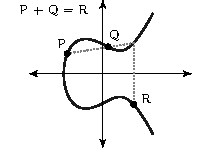
\includegraphics[width=8cm]{tangent-and-chord}
		\caption{``tangent-and-add'' methode op een elliptische kromme\label{figuur-pairings-tangent-and-chord}}
\end{figure}

Aan de hand van de vorige bewerking kan een scalaire vermenigvuldiging vastgelegd worden, met $a \in \mathbb{Z}$:
\[\begin{aligned}
a \cdot A	&= A + \ldots + A\\
0 \cdot A	&= \mathcal{O}\\
-a \cdot A	&= a \cdot -A
\end{aligned}\]

De orde $n$ van een punt $A$ op de kromme is gelijk aan de minimum waarde waarvoor $n \cdot A = \mathcal{O}$. Het is mogelijk dat $n = \infty$. Van alle punten waarvoor $n$ een deler is van $l$ wordt gezegd dat ze in de $l$-torsiesubgroep van $E$ zitten. Zo een subgroep wordt genoteerd als:
\[E[l] = \{ A \in E : l \cdot A = \mathcal{O} \}.\]

Het aantal punten $\#E$ op $E$ wordt de orde van de kromme genoemd. Voor een kromme over een veld $\mathbb{F}_q$ is $\#E = q + 1 - t$, met $t$ de ``trace'' van de kromme. Indien $q \mid t$ wordt de kromme supersingulier genoemd. Voor bepaalde types krommen bestaat er een gesloten formule voor $\#E$.

Ten slotte wordt nog de inbeddingsgraad $k$ gedefinieerd als het kleinste gehele getal waarvoor $n \mid q^k - 1$.

\section{Definitie van pairings}

Een pairing is in dit geval een functie $f(A, B)$ met als argumenten twee punten uit een additieve groep en als resultaat een punt in een multiplicatieve groep:
\[f(A, B): \mathbb{G}_1 \times \mathbb{G}_2 \mapsto \mathbb{G}_T.\]
Een pairing moet tevens volgende eigenschappen bezitten: bilineariteit, non-degeneratie en moet goed gedefinieerd zijn. De betekenis van deze drie begrippen is:

\begin{enumerate}
	\item Bilineariteit: $\forall A_1, A_2, A \in \mathbb{G}_1$ en $\forall B_1, B_2, B \in \mathbb{G}_2$ geldt $f(A_1 + A_2, B) \equiv f(A_1, B) \cdot f(A_2, B)$ en $f(A, B_1 + B_2) \equiv f(A, B_1) \cdot f(A, B_2)$.

	\item Non-degeneratief: $\forall A \in \mathbb{G}_1, \: \exists B \in \mathbb{G}_2$ waarvoor $f(A, B) \neq 1$.

	\item Goed gedefinieerd: $\forall B \in \mathbb{G}_2$ is $f(A, B) = 1$ als en slechts als $A = \mathcal{O}$.
\end{enumerate}

Het zijn de drie eigenschappen waaraan pairings moeten voldoen die het zo moeilijk maken ze te genereren. Ten tijde van dit schrijven waren onder meer volgende pairings bekend: Weil, Tate, $\eta_T$ \cite{eta} en Ate \cite{ate}. In deze thesis zal gewerkt worden met de Tate pairing, waarvan bewezen is dat ze effici\"enter te berekenen is dan de Weil pairing.

De vermelde $\eta_T$ en Ate pairing zijn variaties op de Tate pairing die gebruikt kunnen worden indien voor specifieke elliptische krommen gekozen wordt. Indien aan de juiste voorwaarden voldaan wordt, zal de schakeling die in het volgende hoofdstuk wordt voorgesteld dus ook gebruikt kunnen worden om deze pairings te berekenen.

De definitie van de Tate pairing over elliptische krommen is als volgt:
\[e(A, B): E(\mathbb{F}_{q^k})[l] \times E(\mathbb{F}_{q^k})/l \cdot E(\mathbb{F}_{q^k}) \mapsto \mathbb{F}_{q^k}^* / (\mathbb{F}_{q^k}^*)^l\]
Het resultaat van de Tate pairing is niet uniek, maar een element van een equivalentieklasse in $\mathbb{F}_{q^k}^* / (\mathbb{F}_{q^k}^*)^l$. Voor twee resultaten $a, b \in \mathbb{F}_{q^k}^*$ geldt $a \equiv b$ als en slechts als er een element $c \in \mathbb{F}_{q^k}^*$ waarvoor $a = bc^l$. Aangezien voor cryptografische toepassingen een uniek resultaat gewenst zal zijn, dient die $n$-de macht weggewerkt te worden. Dit kan door het resultaat te verheffen tot de macht $\frac{q^k - 1 }{l}$. Aangezien $a^{q^k - 1} = 1$ voor elke $a \in \mathbb{F}_{q^k}^*$ (kleine stelling van Fermat), verkrijgt men dan dus een $l$-eenheidswortel. Soms wordt over de gereduceerde Tate pairing gesproken wanneer men expliciet wil aangeven dat deze machtsverheffing wordt uitgevoerd.

Het formeel bewijzen van de Tate pairing valt buiten het bestek van deze thesis. Voor meer informatie wordt onder andere verwezen naar \cite{maas, ruck, hess}.

\section{Berekening van de Tate pairing\label{sectie-pairings-berekening}}

Reeds in 1986 stelde Miller een methode voor om de Tate pairing te berekenen \cite{miller, barreto-efficient}. \refalg{algoritme-pairings-miller} geeft weer hoe dat algoritme in z'n werk gaat.

\begin{algorithm}[h]
	\caption{Millers algoritme voor de Tate pairing}
	\label{algoritme-pairings-miller}
	\KwIn{$l \in \mathbb{Z}$; $P, Q \in \mathbb{F}_{q^k}$}
	\KwOut{$e(P, Q) \in \mathbb{F}_{q^k}^*$}
	\KwData{$i, t \in \mathbb{Z}$; $F, S, V \in \mathbb{F}_{q^k}$}
	$t \gets \left\lfloor \log _2 (l) \right\rfloor$\;
	$Q' \gets \textsf{rand}(E)$\;
	$S \gets Q + Q'$\;
	$F \gets 1$; $V \gets P$\;	
	\For{$i = t - 1$ to $0$}{
		$F \gets F^2 \cdot \frac{G_{V,V}(S) \cdot G_{2 \cdot V}(Q')}{G_{2 \cdot V}(S) \cdot G_{V,V}(Q')}$\;
		$V \gets 2 \cdot V$\;
		\If{$m_i = 1$}{
			$F \gets F \cdot \frac{G_{V,P}(S) \cdot G_{V + P}(Q')}{G_{V + P}(S) \cdot G_{V,P}(Q')}$\;
			$V \gets V + P$\;
		}
	}
	\KwRet{$F^{\frac{q^k - 1 }{l}}$}
\end{algorithm}

Daarbij staat $G_{A, B}(C)$ voor de evaluatie van het punt $C$ in de vergelijking van de rechte door de punten $A$ en $B$. Indien $G_{2 \cdot A}$ vermeld staat, wil dit de vergelijking door de raaklijn aan $2 \cdot A$ zeggen.

Hoewel als argumenten van het algoritme elementen van $\mathbb{F}_{q^k}$ staan aangegeven, zal doorgaans voor elementen uit het subveld $\mathbb{F}_q$ gekozen worden. Het resultaat van de pairing zal dus $k$ keer groter zijn dan de opgegeven argumenten. 

In \cite{barreto-efficient} wordt aangetoont dat, mits het gebruik van de supersinguliere kromme
\[E: y^3 + y = x^3 + x + b,\]
het algoritme sterk vereenvoudigd kan worden. Er dient dan een distortiemap $\phi$ toegepast te worden op het punt $Q$. Voor een veld $\mathbb{F}_{2^m}$ dient de mapping te voldoen aan volgende voorwaarden:
\[\phi : (x_Q, y_Q) \mapsto (x_Q + s^2, y_Q + x_Q s + t^6)\]
met $s, t \in \mathbb{F}_{2^{km}}$. Daarbij moeten $s$ en $t$ voldoen aan volgende vergelijkingen:
\[\left\{\begin{array}{l}
s^4 + s = 0\\
t^2 + t + s^6 + s^2 = 0
\end{array}\right.\]

Een tweede voordeel van het gebruik van de vermelde kromme is haar lage inbeddingsgraad $k = 4$. Hoe groter $k$, hoe meer bewerkingen het immers kost om de pairing te berekenen.

Met deze parameters vastgelegd, kan Millers algoritme vereenvoudigd worden tot \refalg{algoritme-pairings-miller-beter}.

\begin{algorithm}[h]
	\caption{Millers algoritme voor de Tate pairing - Effici\"entere versie}
	\label{algoritme-pairings-miller-beter}
	\KwIn{$l \in \mathbb{Z}$; $P, Q \in \mathbb{F}_{2^m}$}
	\KwOut{$e(P, Q) \in \mathbb{F}_{2^{km}}^*$}
	\KwData{$i, t \in \mathbb{Z}$; $F, S, V \in \mathbb{F}_{2^{km}}$}
	$t \gets \left\lfloor \log _2 (l) \right\rfloor$\;
	$F \gets 1$; $V \gets P$\;	
	\For{$i = t - 1$ to $0$}{
		$F \gets F^2 \cdot G_{V,V}(\phi(Q))$\;
		$V \gets 2 \cdot V$\;
		\If{$m_i = 1$}{
			$F \gets F \cdot G_{V,P}(\phi(Q))$\;
			$V \gets V + P$\;
		}
	}
	\KwRet{$F^{\frac{2^{km} - 1 }{l}}$}
\end{algorithm}

\section{Toepassingen van pairings}

Nu de wiskundige achtergrond van de Tate pairing enigszins verduidelijkt is, zullen enkele voorbeelden gegeven worden van het gebruik ervan.
